\graphicspath{{chapters/loadings/}}


\chapter{Insights From Generating Simulated Data for CCA}\label{ch:loadings}
% \epigraph{All models are wrong, some are useful.}{\textit{G. Box}}
\minitoc
% chktex-file 44
% chktex-file 3
\section*{Preface}

This chapter, deriving insights from various projects, lays out both my arguments for the use of loadings in the interpretation of CCA models and a number of computational tricks that we used to generate simulated data with significantly higher dimensions than have been previously considered in the literature.
The simulated data generation methods were used to generate simulated data in \citet{mihalik2022canonical}.
The arguments for the use of loadings influenced our choice of loadings for the interpretation of the results in \citet{ADAMS2024}.

\section{Introduction}

Despite its popularity, there is an ongoing debate in the CCA literature regarding the interpretation of model weights versus loadings \citep{gu2018simultaneous}. This chapter aims to contribute to this debate by providing mathematical insights from generative models of CCA and empirical results from simulated data with higher dimensionality than previously considered in the literature.

We begin by categorizing methods for generating CCA simulated data into explicit and implicit latent variable models. This categorization allows us to compare and contrast the generative models in CCA literature with the generative model for linear regression. We highlight that in linear regression, regularization can be interpreted as a prior on the weights, whereas in CCA, it is perhaps more natural to interpret regularization as a prior on the loadings. By leveraging computational tricks, we demonstrate how to generate simulated data with significantly higher dimensions than previously considered in the literature \citep{helmer2020stability, matkovivc2023static}.

Furthermore, we rigorously prove that loadings are invariant to columnwise transformations in data matrices, unlike weights. This property makes CCA unique compared to Principal Component Analysis (PCA) or Partial Least Squares (PLS) and is particularly relevant in fields like brain-behavior studies, where data preprocessing often involves columnwise manipulation.

Our experimental design focuses on two main aspects. First, we evaluate the ability of CCA models to accurately recover the true model weights and loadings. Second, we examine the out-of-sample performance, which is often observed to be poor in practical datasets despite statistical significance, particularly for PLS-based models. This observation led us to question whether the issue lies in poor model fit or a lack of signal in the data with weak or biologically spurious correlations.

One of our most striking findings, consistent with the previous chapter, is the efficacy of Ridge Regularized CCA models compared to PLS models in identifying high correlations under anisotropic noise conditions; where the noise covariance matrices ($\Psi$) are not scalar multiples of the identity matrix, leading to non-spherical noise distributions. This complements earlier work \citep{helmer2020stability} that found that the number of samples needed to find high correlations increases with dimensionality; our results suggest that the important variable is the dimensionality of the smaller view.

Through this chapter, we aim to provide a comprehensive understanding of the relationship between weights and loadings in CCA models, the impact of regularization on model interpretation, and the performance of CCA models in high-dimensional settings. By unifying generative perspectives, proving mathematical properties, and conducting extensive simulations, we contribute to the ongoing debate in the CCA literature and provide valuable insights for researchers and practitioners applying CCA in various domains.

\section{Background: Weights and Loadings in Canonical Correlation Analysis}

CCA can be interpreted in two ways: either as a method that finds linear combinations of variables in two datasets that exhibit the highest correlation, or as a technique that estimates latent variables that are maximally correlated.

The concept of latent variables is particularly important in biomedical applications, as it can help uncover underlying factors influencing observable data. For example, in brain-behavior studies, latent variables may represent hidden neurological or cognitive processes that drive the relationship between brain structure or function and behavioral outcomes. Similarly, in imaging-genetics, latent variables can capture the genetic factors that influence brain morphology or activity patterns. By introducing latent variables, CCA enables researchers to gain a deeper understanding of complex phenomena like gene expression, pathologies, and normative variations in health-related data \citep{lawry2023multi}.

\subsection{Generative and Discriminative Approaches in CCA}

CCA's practical application revolves around two main approaches: the discriminative approach and the generative approach. 
The generative approach, known as the `forward model', emphasizes the data generation process and employs loadings to describe the relationship between latent variables and observed data. It models the joint distribution of the observed data conditioned on the latent variables, expressed as $P(X\sps{1},X\sps{2}|Z)$. In this approach, the latent variables are assumed to be the underlying cause\footnote{Used here very loosely to give intuition} of the observed data, and the goal is to learn the parameters of the generative model that best explains the data.

In contrast, the discriminative approach, represented as the `backward model' in Figure~\ref{fig:forward-backward-models}, uses weights to estimate highly correlated latent variables from observed data. It focuses on modeling the conditional distribution of the latent variables given the observed data, denoted as $P(Z|X\sps{1},X\sps{2})$. The discriminative approach aims to find the optimal linear combinations of the observed variables that maximize the correlation between the latent variables, without explicitly modeling the data generation process.

\begin{figure}
    \centering
    \tikz{
    % nodes
        \node[latent, align=center, minimum size=2cm] (Z) {Severity\\z};
        \node[obs, below left=of Z, minimum size=2cm, align=center] (x1) {Brain\\$x^{(1)}$};
        \node[obs, below right=of Z, minimum size=2cm, align=center] (x2) {Behaviour\\$x^{(2)}$};
        % edges
        \edge[blue]{Z} {x1};
        \edge[blue]{Z} {x2};
        \edge[red, tension=0.1]{x1} {Z};
        \edge[red, tension=0.1]{x2} {Z};
    }
    \caption[Forward and Backward Multiview Models]{\textit{\textbf{Forward and Backward Multiview Models:}} The \textcolor{blue}{generative/forward} and \textcolor{red}{discriminative/backward} approaches in \acrshort{cca}.}\label{fig:forward-backward-models}
\end{figure}

\subsection{Analogy Between CCA and PCA}

The distinction between the generative and discriminative approaches in CCA is analogous to the different interpretations of Principal Component Analysis (PCA) \citep{park2023critical}. PCA can also be viewed from a generative perspective, where the observed data are assumed to be generated from latent variables \citep{tipping1999probabilistic}, or from a discriminative perspective, where the principal components are linear combinations of the observed variables that maximize the variance \citep{hotelling1933analysis}.

In both CCA and PCA, the generative approach focuses on modeling the joint distribution of the observed data and the latent variables, while the discriminative approach emphasizes finding the optimal linear combinations of the observed variables to estimate the latent variables or principal components.

\subsection{The Debate Regarding Weights and Loadings in CCA}

In CCA research, there is an ongoing debate regarding the interpretation of models in terms of weights or loadings \citep{gu2018simultaneous}. Weights are often preferred for prediction tasks, as they directly relate the observed variables to the latent variables. On the other hand, loadings are favored for interpretation, as they provide insights into the structure and relationships within the data \citep{liu2022improved}. This discussion is particularly relevant to our work in chapter \ref{ch:als} and various studies involving sparse CCA and sparse Partial Least Squares (PLS), where understanding the meaning and implications of sparse loadings and weights is crucial.

Given the importance of this topic, especially in the context of our work in chapter \ref{ch:als} and other studies employing variants of sparse CCA and sparse PLS, it is essential to delve deeper into the interpretation of sparse loadings and weights. In the following sections, we will explore the mathematical properties and practical implications of weights and loadings in CCA, with a focus on sparse and regularized models. By addressing this key aspect of CCA, we aim to contribute to the ongoing debate and provide insights that can guide the application and interpretation of CCA in various domains, including neuroimaging, genetics, and health-related research.

\section{Methods: Unifying Generative Perspectives in CCA: Explicit and Implicit Latent Variable Models of Multiview Data}

This section categorizes the generative models in CCA literature into explicit and implicit latent variable types, each offering distinct insights into the data generation process and the relationship between weights and loadings.

\subsection{Additional Notational Conventions}

We will use some additional notational convention to describe probabilistic models.
We will use lowercase letters to represent samples from a distribution, and uppercase letters to represent random variables.
For example, \(x\) represents a sample from the distribution \(P(X)\), and \(X\) represents the random variable \(X\).
We will use $\sim$ to denote the sampling process, and $|$ to denote conditioning.
For example, \(x | z \sim \mathcal{N}(\mu, \Psi)\) represents a sample \(x\) from a Gaussian distribution with mean \(Wz\) and covariance \(\Psi\) conditioned on the latent variable \(z\).
We also introduce the notation \(w\sps{i}_{j}\) to refer to the loading of the \(j\)-th feature in the \(i\)-th view on a latent variable, as well as \(W\sps{i}\) to refer to the matrix of loadings for the \(i\)-th view on all latent variables.

\subsection{Explicit Latent Variable Models: Probabilistic CCA and Group Factor Analysis}

Explicit latent variable models assume that the observed data in each view is generated from a shared latent space, with view-specific linear transformations and added noise. These models provide a probabilistic framework for understanding the relationship between multiple views of data and the underlying latent factors that give rise to them.

\subsubsection{Probabilistic CCA}
Probabilistic CCA (PCCA) is an explicit latent variable model that extends classical CCA to a probabilistic setting. In PCCA, the generative process for two views can be described as follows:
\begin{align}
z &\sim \mathcal{N}(0, I)\\
x\sps{i} &\sim \mathcal{N}(W\sps{i} z + \mu\sps{i}, \Psi\sps{i})
\end{align}
where $z$ is a shared latent variable drawn from a standard normal distribution, $x\sps{i}$ represents a sample from the $i$-th view, $W\sps{i}$ are the view-specific loadings that map the latent space to the observed space, $\mu\sps{i}$ is the mean of the $i$-th view, and $\Psi\sps{i}$ is the view-specific noise covariance matrix.

The key idea behind PCCA is that the shared latent variable $z$ captures the common structure across views, while the view-specific loadings $W\sps{i}$ allow for flexibility in how this structure is expressed in each view. The noise covariance matrices $\Psi\sps{i}$ account for view-specific variation not explained by the shared structure.
\citet{bach2005probabilistic} showed that the maximum likelihood estimates of the loadings $W\sps{i}$ in PCCA are related to the classical CCA weights $U\sps{i}$ by the within-view covariance matrices $\Sigma_{ii}$:
\begin{align}\label{eq:weights-to-loadings}
W\sps{i} &= \Sigma_{ii} U\sps{i} R\\
U\sps{i} R &= \Sigma_{ii}^{-1} W\sps{i}
\end{align}
where $R$ is an arbitrary rotation matrix. This result provides a link between the probabilistic and non-probabilistic formulations of CCA, and suggests that the classical CCA weights can be interpreted as estimates of the true loadings, up to a rotation.
\subsubsection{Group Factor Analysis}
Group Factor Analysis (GFA) \citep{klami2014group} is another explicit latent variable model that extends PCCA by assuming isotropic (i.e., spherical) noise in each view:
\begin{align}
z &\sim \mathcal{N}(0, I)\
x\sps{i} &\sim \mathcal{N}(W\sps{i} z + \mu\sps{i}, \sigma_i^2 I)
\end{align}
where $\sigma_i^2$ is the noise variance in the $i$-th view. This assumption simplifies the model and can lead to computational benefits, as well as supporting extensions like sparsity on the loadings.
The joint distribution of multiple views under the GFA model is a multivariate Gaussian distribution with a structured covariance matrix:
\begin{align}
\begin{bmatrix}
X\sps{1} \ \vdots \ X\sps{m}
\end{bmatrix} \sim \mathcal{N} \left( \begin{bmatrix}
\mu\sps{1} \ \vdots \ \mu\sps{m}
\end{bmatrix}, \begin{bmatrix}
W\sps{1}W\spsT{1} + \sigma_1^2 I & \cdots & W\sps{1}W\spsT{m} \\
\vdots & \ddots & \vdots \\
W\sps{m}W\spsT{1} & \cdots & W\sps{m}W\spsT{m} + \sigma_m^2 I
\end{bmatrix} \right)
\end{align}
This highlights the fact that the covariance structure in each view is determined by the view-specific loadings and noise variances. When the loadings $W\sps{i}$ have large singular values compared to the noise variances $\sigma_i^2$, the resulting covariance matrices $\Sigma_{ii} = W\sps{i}W\spsT{i} + \sigma_i^2 I$ are often referred to as "spiked covariance matrices" \citep{johnstone2001distribution}.

\subsubsection{Connecting GFA and Probabilistic PCA}
Probabilistic PCA (PPCA) \citep{tipping1999probabilistic} is a special case of GFA applied to a single view:
\begin{align}
z &\sim \mathcal{N}(0, I)\\
x &\sim \mathcal{N}(W z + \mu, \sigma^2 I)
\end{align}
Like GFA, PPCA assumes isotropic noise and seeks to identify a lower-dimensional latent space that captures the structure in the observed data. The key difference is that PPCA does not model multiple views or the relationships between them.
However, the connection between GFA and PPCA provides an important insight: when the noise in each view is low and isotropic, the shared latent structure dominates the view-specific noise. In this scenario, applying PPCA to a single view should recover latent variables that are very similar to those obtained by applying GFA to multiple views.
This suggests that, in low-noise settings, it may be possible to uncover meaningful latent structure using just a single view of the data. Consequently, PPCA can serve as a useful baseline for evaluating the performance of multi-view models like GFA. Likewise in the discriminative setting, if a multi-view model does not significantly outperform PCA applied to a single view, it may indicate that the additional complexity of the multi-view approach is not justified for that particular dataset.
For this reason, it is always my reccomendation to compare the performance of multi-view models to that of PCA applied to each individual view\footnote{In the growing Deep Multiview Learning literature this is analagous to comparing to separate autoencoders applied to each view}. This can help assess whether the multi-view approach is truly leveraging complementary information across views, or if the observed performance gains are due to other factors, such as noise reduction or increased model capacity.
By understanding the relationships between these explicit latent variable models, researchers can make more informed decisions about when and how to apply them to real-world datasets, and can better interpret the results obtained from multi-view analyses.

\subsection{Implicit Latent Variable Models: The Joint Covariance Matrix Perspective}

The joint covariance matrix perspective, prevalent in sparse CCA literature \citep{suo2017sparse,chen2013sparse}, emphasizes covariance matrices over direct modeling of latent variables.
This approach allows us to directly control the sparsity of the weights and the strength of the canonical correlations by constructing the covariance matrices accordingly. By focusing on the covariance structure, we can generate data with desired properties without explicitly modeling the latent variables.
This is achieved by constructing the joint covariance matrix of the distribution \(P(X\sps{1},X\sps{2})\):

\begin{align}
    \begin{bmatrix}
        X\sps{1} \\ X\sps{2}
    \end{bmatrix} \sim \mathcal{N} \left( \begin{bmatrix}
                                              0 \\ 0
    \end{bmatrix}, \begin{bmatrix}
                       \Sigma_{11} & \Sigma_{12} \\ \Sigma_{21} & \Sigma_{22}
    \end{bmatrix} \right)
\end{align}

Where \(\Sigma_{11}\) and \(\Sigma_{22}\) are the within-view covariance matrices and \(\Sigma_{12}\) and \(\Sigma_{21}\) are the between-view covariance matrices.

For clarity and simplicity in our discussion, we refer to a single canonical correlation coefficient, \(\rho\), without loss of generality.
This allows us to focus on the structure of the covariance matrices without the complexity of multiple canonical correlations.

In constructing the between-view covariance matrices \(\Sigma_{12}\) and \(\Sigma_{21}\), we control the true signal by setting active variables and correlations.
Specifically, the between-view covariance matrix is constructed as follows:

\begin{align}
    \Sigma_{12} = \rho \Sigma_{11} u\sps{1}_{1} u\spsT{2}_{1} \Sigma_{22}
\end{align}
%
Here, \(\rho\) is the canonical correlation, and \(u\sps{i}_{1}\) is the first column of the matrix of weights \(U\sps{i}\) for the \(i\)-th view.

This perspective simplifies the structure of covariance matrices, focusing on the relationship between views as controlled by the canonical correlation coefficient, \(\rho\), and the weights \(u\sps{i}\).

\subsection{Noise Structures and Their Impact on Covariance Modeling}
The noise covariance matrices $\Psi\sps{i}$ in the explicit latent variable models play a crucial role in determining the nature of the noise in each view. When the noise covariance matrix is a scalar multiple of the identity matrix, i.e., $\Psi\sps{i} = \sigma_i^2 I$, the noise is considered isotropic or spherical, with equal variance in all dimensions and no correlations. On the other hand, when the noise covariance matrix is not a scalar multiple of the identity matrix, the noise is considered anisotropic or non-spherical, with potentially different variances across dimensions and correlations between noise components.
In real-world datasets, such as those involving brain and behavioral data, the assumption of isotropic noise may not always hold. The correlation between brain regions or behavioral measures refers to the structured relationships in the data, captured by the loadings $W\sps{i}$ in the explicit latent variable models. The noise, on the other hand, represents the unstructured variation or measurement error not explained by the latent factors. While brain regions and behavioral measures may be correlated due to shared underlying processes, this does not necessarily imply that the noise itself is correlated.
When analyzing brain and behavioral data using explicit latent variable models or related methods, it is important to consider the potential for both correlated and uncorrelated noise structures. Ignoring the possibility of correlated noise and assuming an identity covariance matrix may oversimplify the noise characteristics, potentially leading to suboptimal results or misinterpretations. Conversely, assuming correlated noise when it is not present can lead to overparameterization and reduced interpretability.
In addition to the noise covariance, the observed covariance structures are also important to consider. Discriminative methods, such as classical CCA, often make assumptions about the observed covariance matrices $\Sigma_{ii}$, taking them as given or estimating them from the data. In contrast, generative methods, such as Probabilistic CCA and GFA, model the observed covariance as a function of the loadings and the noise covariance, as shown in Table \ref{tab:covariance-structures}.
Researchers should carefully examine the properties of the data and use prior knowledge about the measurement process to guide their assumptions about both the noise and observed covariance structures. Comparing models with different assumptions (e.g., isotropic vs. anisotropic noise, identity vs. non-identity observed covariance) and using model selection techniques can help determine the most appropriate choice when the covariance structures are uncertain. By considering the potential for different noise and observed covariance structures, researchers can make more informed decisions about the modeling assumptions and improve the accuracy and interpretability of their results.

\subsection{Summary of Data Generation Methods}

To summarize the key differences between the data generation methods discussed above, we present two tables. Table \ref{tab:covariance-structures} compares the covariance structures of each method, highlighting how the within-view and between-view covariances are modeled. Table \ref{tab:weights-loadings-population-sample} illustrates the relationship between weights and loadings in both population and sample cases, emphasizing the implications for sparsity and identifiability.

\renewcommand{\arraystretch}{2.5} % Increase the row height
\begin{table}[h]
    \centering
    \caption{Covariance Structures in Data Generation Methods}
    \begin{tabular}{|c|c|c|c|}
        \hline
        \textbf{}                                           & \textbf{Method}              & \textbf{Within-view Covariance} $\boldsymbol{\Sigma_{ii}}$ & \textbf{Between-view Covariance} $\boldsymbol{\Sigma_{12}}$ \\
        \hline
        \multirow{2}{*}{\rotatebox[origin=c]{90}{Explicit}} & Probabilistic \acrshort{cca} & $W\sps{i}W\spsT{i} + \Psi\sps{i}$ & $W\sps{1}W\spsT{2}$ \\
        \cline{2-4}
        & \acrshort{gfa}               & $W\sps{i}W\spsT{i} + {\sigma\sps{i}}^2 I$                    & $W\sps{1}W\spsT{2}$                                                 \\
        \hline
        \multirow{2}{*}{\rotatebox[origin=c]{90}{Implicit}} & Joint Covariance             & $\Sigma_{ii}$ & $\rho \Sigma_{11}u\sps{1}_1 u\spsT{2}_1 \Sigma_{22}$ \\
        \cline{2-4}
        & Joint Covariance (Identity)  & $I$                                                        & $\rho u\sps{1}_1 u\spsT{2}_1$                       \\
        \hline
    \end{tabular}
    \label{tab:covariance-structures}
\end{table}

As shown in Table \ref{tab:covariance-structures}, the explicit latent variable models (Probabilistic CCA and GFA) incorporate the noise covariance matrices $\Psi\sps{i}$ or $\sigma_i^2 I$ into the within-view covariance expressions. This allows for more flexible modeling of the noise structure, as the noise covariance can be either isotropic (in the case of GFA) or anisotropic (in the case of Probabilistic CCA). In contrast, the implicit latent variable models (Joint Covariance) assume a simpler noise structure, often taking the within-view covariance matrices $\Sigma_{ii}$ as given or assuming an identity covariance for tractability.

Table \ref{tab:weights-loadings-population-sample} summarizes the relationship between the weights and loadings in each data generation method, distinguishing between population and sample cases.
This distinction is crucial, especially in scenarios where the population covariance matrix \( \Sigma \) is identity, but the sample covariance matrix \( \hat{\Sigma} \) is only an approximation.
An important observation is that for the implicit latent variable models, we can generate data with sparse weights but not, in general, sparse loadings.
For the explicit latent variable models, we can generate data with sparse loadings but not, in general, sparse weights.

\begin{table}[h]
    \centering
    \caption{Relationship Between Weights and Loadings in Population and Sample Cases}
    \begin{tabular}{|c|c|c|c|c|}
        \hline
        \textbf{}                                           & \textbf{Method}                 & \textbf{Case} & \textbf{Weights}                            & \textbf{Loadings}                \\
        \hline
        \multirow{4}{*}{\rotatebox[origin=c]{90}{Explicit}} & Probabilistic \acrshort{cca} & Population & $(W\sps{i}W\spsT{i} + \Psi\sps{i})^{-1}W\sps{i}$ & $W\sps{i}$ \\
        &                                 & Sample        & $\hat{\Sigma_{ii}}^{-1}W\sps{i}$             & $W\sps{i}$                        \\
        \cline{2-5}
        & \acrshort{gfa}                  & Population    & $(W\sps{i}W\spsT{i} + {\sigma\sps{i}}^2 I)^{-1}W\sps{i}$      & $W\sps{i}$                        \\
        &                                 & Sample        & $\hat{\Sigma_{ii}}^{-1}W\sps{i}$             & $W\sps{i}$                        \\
        \hline
        \multirow{4}{*}{\rotatebox[origin=c]{90}{Implicit}} & Joint Covariance (Non-Identity) & Population & $U\sps{i}$ & $\Sigma_{ii}U\sps{i}$ \\
        &                                 & Sample        & $U\sps{i}$                                   & $\hat{\Sigma_{ii}}\hat{U\sps{i}}$ \\
        \cline{2-5}
        & Joint Covariance (Identity)     & Population    & $U\sps{i}$                                   & $U\sps{i}$                        \\
        &                                 & Sample        & $U\sps{i}$                                   & $\hat{\Sigma_{ii}}\hat{U\sps{i}}$ \\
        \hline
    \end{tabular}
    \label{tab:weights-loadings-population-sample}
\end{table}

\subsection{Regularization and Generative Models}

Regularization is crucial in CCA to prevent overfitting and promote interpretability. However, the way regularization is interpreted in CCA differs from linear regression due to the latent variable nature of CCA models. In linear regression, regularization can be directly interpreted as a prior on the weights. In contrast, for CCA, regularization can be interpreted as a prior on either the loadings or the weights, depending on the generative perspective. This distinction has important implications for model interpretation and the identifiability of weights in CCA.

\subsubsection{Regularization and the Generative Model for Linear Regression}
Linear regression assumes data generation from a linear model with added noise:

\begin{align}
    y = xU + \epsilon, \quad \epsilon \sim \mathcal{N}(0, \sigma^2 I)
\end{align}

Here, $y$ are samples of the target variable, $x$ samples from the data matrix, $U$ the regression coefficients, and $\epsilon$ represents independent and identically distributed (i.i.d.) Gaussian noise.

\paragraph{Lasso Regression}
The Lasso imposes a Laplace prior on the regression coefficients, leading to a double-exponential prior on weights:

\begin{align}
    U \sim \mathcal{L}(0, \lambda)
\end{align}

\paragraph{Ridge Regression}
Ridge regression, in contrast, employs a Gaussian prior on the regression coefficients, equivalent to a Gaussian prior on weights:

\begin{align}
    U \sim \mathcal{N}(0, \lambda)
\end{align}

\subsubsection{Regularization and Generative Models for CCA}
CCA models differ in their approach to regularization compared to linear regression because they are latent variable models.

\paragraph{Explicit Latent Variable Model}
Regularization in the context of the explicit latent variable naturally relates to priors on the loadings \(W\sps{i}\).
For example, sparsity in the loadings can be achieved by imposing a Laplace prior on the loadings:

\begin{align}
    W\sps{i} \sim \mathcal{L}(0, \lambda)
\end{align}

This expresses the prior belief that latent factors only explain the data through a small number of features.
For example, in the context of latent factors in brain-behavior studies, this prior belief is equivalent to the assumption that a latent mode of variance (perhaps a subtype) is only expressed through a small number of brain regions.

\paragraph{Implicit Latent Variable Model}
In the implicit latent variable model of CCA, the joint likelihood is modeled as a block covariance matrix \(\Sigma\)\citep{suo2017sparse}, constructed from the weights \(U\sps{i}\).

\begin{equation}
    \Sigma = \begin{bmatrix}
                 \Sigma_{1} & \Sigma_{1} U\sps{1} \rho U\spsT{2} \Sigma_{2} \\
                 \Sigma_{2} U\sps{2} \rho U\spsT{1} \Sigma_{1} & \Sigma_{2}
    \end{bmatrix}
\end{equation}

Where the off-diagonal blocks \(\Sigma_{1} U\sps{1} \rho U\spsT{2} \Sigma_{2}\) and its transpose represent the between-view covariance matrices.
These matrices are functions of the weights \(U\sps{i}\) and within-view covariance matrices \(\Sigma_{i}\), modulated by \(\rho\), the canonical correlation coefficients.

Here the regularization naturally relates to priors on the weights \(U\sps{i}\).
For example, sparsity in the weights can be achieved by imposing a Laplace prior on the weights:

\begin{align}
    U\sps{i} \sim \mathcal{L}(0, \lambda)
\end{align}

This expresses the more nuanced prior belief that the latent factors are expressed through a subset of features and then distorted by arbitrary rotations as well as the within-view covariance matrices.
Manipulating equation \ref{eq:weights-to-loadings}, the conditional distribution of the implicit latent variable model we have:

\begin{align}
    x\sps{i} | z &\sim \mathcal{N}(\Sigma_{i}U\sps{i}R z=W\sps{i}z, \Sigma_{i}-W\sps{i}W\spsT{i}=\Psi\sps{i}) \\
    z &\sim \mathcal{N}(0, I)
\end{align}

The arbitrary rotation matrix \(R\) means that for multidimensional $U\sps{i}$, even if $\Sigma_{i}=I$, and even if the true loadings are sparse, the weights may still not be sparse!

\begin{align}
    x\sps{i} | z &\sim \mathcal{N}(U\sps{i}R z=W_{sparse}\sps{i}z, \Sigma_{i}-W_{sparse}\sps{i}W_{sparse}\spsT{i}=\Psi\sps{i}) \\
    z &\sim \mathcal{N}(0, I)
\end{align}

Alternatively, even if we know the true weights (i.e. $R=I$), the CCA model may not be able to recover them.
This is to say they are not, in general, identifiable \citep{park2023critical}.
In other words there are multiple values of $W\sps{i}$ that can produce the same covariance structure.

We can illustrate this with a trivial example:

\begin{align}
    \Sigma_{1} &= \begin{bmatrix}
                         1 & 1 & 0 \\
                         1 & 1 & 0 \\
                         0 & 0 & 1
    \end{bmatrix}\begin{bmatrix}
                     1 \\
                     0 \\
                     1
    \end{bmatrix}=
    \begin{bmatrix}
        1 & 1 & 0 \\
        1 & 1 & 0 \\
        0 & 0 & 1
    \end{bmatrix}\begin{bmatrix}
                     0.5 \\
                     0.5 \\
                     1
    \end{bmatrix}= \begin{bmatrix}
                        1 \\
                        1 \\
                        1
    \end{bmatrix} \\
\end{align}

In this example, we show that the same covariance matrix $\Sigma_1$ can be obtained using different weight matrices. The first weight matrix has entries [1, 0, 1], while the second weight matrix has entries [0.5, 0.5, 1]. This example clearly demonstrates the non-identifiability issue in the implicit latent variable model, where multiple weight matrices can produce the same covariance structure. This means that even if we know the true covariance structure, we may not be able to uniquely recover the true weights.

One practical implication of this observation is that it raises serious questions about using stability selection, a common practice in the sparse \acrshort{cca} literature \citep{mihalik2020multiple, deng2021sparse}, to select the optimal regularization parameter.For instance, suppose we run stability selection multiple times on the same dataset to select the optimal regularization parameter. Due to the non-identifiability of weights, each run may result in different rotations of the weights, even though the underlying representations and correlations remain the same. This can lead to inconsistent selection of the regularization parameter across runs, potentially resulting in suboptimal hyperparameter choices or incorrect conclusions about the sparsity structure of the data.

In summary, understanding the generative perspectives in CCA is crucial for interpreting regularization, sparsity, and identifiability in these models. The explicit latent variable model allows for intuitive priors on the loadings, while the implicit latent variable model enables priors on the weights, albeit with less straightforward interpretations. The non-identifiability issue in the implicit model highlights the challenges in recovering unique weights and raises questions about the reliability of stability selection. By considering these generative perspectives, researchers can make more informed choices when applying regularization and interpreting the results of CCA models.

\section{Invariance of Loadings in CCA: An Intuitive Mathematical Argument}

In this section, we present an intuitive mathematical argument for favoring loadings over weights in the interpretation of CCA models. We will demonstrate that loadings are invariant to certain common transformations of the data matrix, including scaling, duplication, and summation of columns. This property is not shared by weights. This invariance has significant practical implications, especially when working with heterogeneous or transformed data.

\subsection{Solving CCA in Principal Component Space}
Consider the singular value decomposition (SVD) of the data matrices:

\begin{align}
X\sps{i} = U\sps{i}S\sps{i}V\spsT{i} \label{eq:svd}
\end{align}

Here, $U\sps{i}$ contains the left singular vectors (principal components) of $X\sps{i}$, $S\sps{i}$ is a diagonal matrix of singular values, and $V\sps{i}$ contains the right singular vectors. The columns of $U\sps{i}$ span the column space of $X\sps{i}$, which is the space of all possible linear combinations of the columns of $X\sps{i}$. Intuitively, the column space captures all the directions in which the data varies.

The CCA objective is to find weights $u\sps{1}, u\sps{2}$ that maximize the correlation between the canonical variables $X\sps{1}u\sps{1}$ and $X\sps{2}u\sps{2}$:

\begin{align}
\max_{u\sps{1}, u\sps{2}} \Corr(X\sps{1}u\sps{1}, X\sps{2}u\sps{2}) &= \max_{u\sps{1}, u\sps{2}} \Corr(U\sps{1}S\sps{1}V\spsT{1}u\sps{1}, U\sps{2}S\sps{2}V\spsT{2}u\sps{2}) \label{eq:cca_obj}
\end{align}

By reparameterizing the weights as $v\sps{i} = S\sps{i}V\spsT{i}u\sps{i}$, we obtain:

\begin{align}
\max_{v\sps{1}, v\sps{2}} \Corr(U\sps{1}v\sps{1}, U\sps{2}v\sps{2}) \label{eq:reparam}
\end{align}

This shows that CCA can be solved entirely in the principal component space spanned by the matrices $U\sps{i}$. The loadings $w\sps{i}_j$, defined as the correlations between the original features $X\sps{i}_j$ and the canonical variables $U\sps{i}v\sps{i}$, capture the relationships in this space.

\subsection{Invariance of Loadings to Data Transformations}

We now show that the loadings are invariant to certain transformations of the data matrix $X\sps{i}$, while the weights are not. The key insight is that these transformations change the right singular vectors $V\sps{i}$ and singular values $S\sps{i}$, but not the left singular vectors $U\sps{i}$. Since the loadings depend only on $U\sps{i}$, they remain invariant. Moreover, these transformations preserve the column space of $X\sps{i}$, which is why the principal components $U\sps{i}$ are unaffected.

\subsubsection{Scaling Transformation}
Consider a diagonal scaling matrix $B$ that scales the columns of $X\sps{i}$:

\begin{align}
\tilde{X}\sps{i} = X\sps{i}B = (U\sps{i}S\sps{i}V\spsT{i})B = U\sps{i}(S\sps{i}B)(V\spsT{i}) \label{eq:scaling}
\end{align}

The weights $\tilde{u}\sps{i}$ in the transformed space are related to the original weights by $\tilde{u}\sps{i} = B^{-1}u\sps{i}$, and thus change with the scaling. However, the principal components $U\sps{i}$ remain unchanged, so the loadings $\tilde{w}\sps{i}_j = \Corr(\tilde{X}\sps{i}_j, U\sps{i}v\sps{i}) = w\sps{i}_j$ are invariant.

\subsubsection{Duplication Transformation}
Consider duplicating columns of $X\sps{i}$ using a transformation matrix $B$ that contains an identity matrix $I_n$ and a duplication matrix $D$:

\begin{align}
B = \begin{bmatrix}
I_n \
D
\end{bmatrix}, \quad
\tilde{X}\sps{i} = X\sps{i}B = U\sps{i}(S\sps{i}B)(V\spsT{i}) \label{eq:duplication}
\end{align}

The weights $\tilde{u}\sps{i}$ become underdetermined in the transformed space due to the added linear dependencies. However, since the column space of $\tilde{X}\sps{i}$ is the same as that of $X\sps{i}$, the principal components $U\sps{i}$ and thus the loadings remain unchanged.

\subsubsection{Linear Combination Transformation}
Consider adding or removing linear combinations of columns using a transformation matrix $B$ that contains an identity matrix $I_n$ and a coefficient matrix $C$:

\begin{align}
B = \begin{bmatrix}
I_n & C
\end{bmatrix}, \quad
\tilde{X}\sps{i} = X\sps{i}B = U\sps{i}(S\sps{i}B)(V\spsT{i}) \label{eq:linear_combination}
\end{align}

As before, the weights $\tilde{u}\sps{i}$ change in the transformed space, but since the column space is preserved, the principal components $U\sps{i}$ and loadings remain invariant.

\subsection{Practical Implications}
The invariance of loadings to data transformations has significant practical implications, especially in fields like biomedical research, psychometrics, and social sciences where questionnaire and survey data are common:
\begin{itemize}
    \item \textbf{Interpretability}: Loadings provide a consistent interpretation of the relationships between the original features and the canonical variables, even if the data is rescaled or transformed. This is particularly valuable in interdisciplinary research, where different data normalization practices may be employed.
    \item \textbf{Feature Selection}: Decisions about including, excluding, or combining features can be made based on the loadings without worrying about their impact on the CCA solution. This is especially relevant when dealing with summary measures that effectively sum other variables, a common scenario in questionnaire and biomedical data. The invariance of loadings to such alterations in the data structure makes them a more robust choice for interpreting relationships between variables in these contexts.
    \item \textbf{Robustness}: CCA models can be trained on transformed data (e.g., normalized or standardized) while still allowing for meaningful interpretation in the original feature space. While the identifiability of weights can be partially solved by the standardization of data, and while this is a common practice, it is not always necessary or desirable and always introduces assumptions.
\end{itemize}

In conclusion, this section provides a strong mathematical foundation for the preference of loadings over weights in the interpretation of CCA models. The invariance of loadings to columnwise transformations, including scaling and linear combinations, ensures a more robust and consistent interpretation of variable relationships. This property is especially valuable in fields dealing with heterogeneous or transformed data, where data preprocessing choices may vary. By focusing on loadings, researchers can obtain more reliable insights into the underlying structure of their data, facilitating cross-disciplinary collaborations and the advancement of knowledge.

\section{Methods: Efficient Sampling of Simulated CCA Data}\label{sec:efficient}

Efficient sampling is crucial for CCA because it allows researchers to work with larger datasets and explore more complex or more nuanced relationships between variables, ultimately expanding the scope of research and analysis. Traditional methods can be computationally intensive and storage-demanding, especially for large datasets.
This has in practice limited the dimensionality of simulated data, restricting the scope of research and analysis.
For example \citet{matkovic2023contribution} simulate data with 8,000 observations and 100 features while \citet{helmer2020stability} used at most 10,000 observations and 64 features.
We were interested in the behavior of CCA in high-dimensional settings like voxel-wise MRI and brain connectivities, which can have hundreds of thousands of features \citep{jack2008alzheimer} and up to tens of thousands of observations \citep{sudlow2015uk}.
By leveraging the assumptions that biomedical data often exhibit low-rank and/or sparse covariance structures, we develop efficient sampling methods that overcome the computational and storage limitations associated with high-dimensional data.

\subsection{Challenges with High-Dimensional Data}
Direct sampling from a multivariate normal distribution is impractically slow for high-dimensional data, which has been a core research challenge for Monte Carlo methods \citep{mackay1998introduction}. The implicit latent variable model, in particular, requires storage of the full covariance matrix, which is prohibitive for high-dimensional data. For example, a covariance matrix with 100,000 dimensions would require 80GB of memory, far exceeding the capacity of most personal computers.

\subsection{Efficient Sampling for Explicit Latent Variable Models}
The explicit latent variable model offers more efficient approaches for sampling high-dimensional data by employing sparse and low-rank covariance matrices.

\subsubsection{Sampling from Multivariate Normal Distributions}
An efficient approach to sampling from a multivariate normal distribution is to use the Singular Value Decomposition (SVD) or Cholesky decomposition of the covariance matrix. This involves decomposing the covariance matrix and using the resulting components to transform samples from a standard multivariate normal distribution:

\begin{align}
Z~\sim \mathcal{N}(0, I) \\
X = \Sigma^{1/2}Z
\end{align}

Where \( \Sigma^{1/2} \) is a square root of the covariance matrix, obtained through SVD or Cholesky decomposition. This is the same as the generative model for the explicit latent variable model, where \( \Sigma^{1/2} \) is the matrix of loadings. Low-rank noise can be added by sampling from an independent multivariate normal distribution and adding it to the transformed samples. This approach requires sampling from a univariate normal distribution and performing a matrix multiplication of complexity \(\mathcal{O}(np^2)\).

\subsubsection{Using Sparse and Low-Rank Covariance Matrices}
Sparse covariance matrices, with many zero entries, reduce both computational complexity and storage requirements. For example, a sparse covariance matrix with 100,000 dimensions and 10\% density would only require 8GB of memory to store.

Low-rank covariance matrices further reduce complexity by storing only the factorized rank-$k$ components, reducing storage requirements to \(\mathcal{O}(kp)\). For example, a low-rank covariance matrix with 100,000 dimensions, 10\% density, and rank 1000 would only require 80MB of memory to store. This approach also requires drawing \(\mathcal{O}(kp)\) samples from a univariate normal distribution and performing a matrix multiplication with complexity \(\mathcal{O}(nkp)\), rather than \(\mathcal{O}(np^2)\) for the full-rank case.

\subsection{Calculating True Canonical Correlations and Weights}
The population canonical correlations can be controlled by varying the signal-to-noise ratio (SNR), i.e., the ratio of the signal variance to the noise variance.

For the explicit latent variable model, the loadings are obtained directly as the low-rank square root of the covariance matrix. The weights can be calculated from the loadings and the covariance matrix using the relationship:

\begin{align}
\hat{W}\sps{i} = \Sigma_{ii} \hat{U}\sps{i} R
\end{align}

Where $R$ is an arbitrary rotation matrix and $\hat{U}\sps{i}$ is the matrix of \acrshort{cca} weights for the $i$th view. For invertible covariance matrices, the `true' \acrshort{cca} weights associated with the top-k subspace can be accessed by multiplying the \gls{loadings} by the inverse of the covariance matrix:

\begin{align}
\hat{U}\sps{i}R = \Sigma_{ii}^{-1} \hat{W}\sps{i}
\end{align}

Although inverting the \(\mathcal{O}(p^2)\) covariance matrix is computationally expensive, the Sherman-Morrison-Woodbury formula can be used to calculate the inverse in \(\mathcal{O}(kp^2)\) time for a rank-$k$ covariance matrix. This allows for the calculation of weights in \(\mathcal{O}(kp^2)\) time, which is faster than the \(\mathcal{O}(p^3)\) time required to calculate the weights directly from the covariance matrix.

In the next section, we will present experiments demonstrating the relationship between weights and \gls{loadings} in simulated data using these efficient sampling techniques.

\section{Experiment Design}

Our goal in this section is to empirically demonstrate the relationship between weights and \gls{loadings} in \acrshort{cca} models as well as to better understand the behavior of \acrshort{cca} models in the high-dimensional settings that section \ref{sec:efficient} enables, and which are of interest in the neuroimaging community.

The first set of experiments illustrates the relationship between weights and \gls{loadings} in simulated data using explicit latent variable models with identity and non-identity covariance matrices.
The second set of experiments illustrates the ammount of information that can be recovered from simulated data using \acrshort{cca} and \acrshort{pls} models with varying signal-to-noise ratios and sample sizes.

\subsection{Exploring the Relationship Between Weights and Loadings in CCA Using Simulated Data}

Our first experiment is designed to illustrate the challenges of recovering the true weights and \gls{loadings} respectively in \acrshort{cca} models for explicit and implicit latent variable models with identity and non-identity covariance matrices.

We compare the true weights derived from the data generation model with the estimated weights of CCA, Ridge CCA, Elastic Net CCA (implemented with FRALS-EN), PLS, and PCA models.
We expect that when the covariance matrix is identity, the weights and \gls{loadings} will be identical.
When the covariance matrix is non-identity, we expect that the weights and \gls{loadings} will be different.
Moreover, we expect that the estimated loadings will be more stable than the estimated weights for CCA models because the weights are not always identifiable.
Under the explicit latent variable model, we expect that the weights will only be (close to) sparse when the covariance matrix is close to identity.
This means we do not expect the Elastic Net CCA model to improve on the Ridge CCA model since the Lasso regularizes the weights but not the \gls{loadings}.
Finally, we expect that when using the explicit latent variable model, for high signal-to-noise ratios, the PLS and even PCA models will recover the true weights and \gls{loadings} because the majority of the variance is explained by the latent variables.

\subsubsection{Detailed Parameters of Simulated Data for Weights and Loadings Analysis in CCA} We generate data with 100 samples and 10 features in each view.
We then generate data under two implicit latent variable models and two explicit latent variable models.
The ridge penalty is coarsely tuned between 0.1 and 0.9 in order to illustrate the effect of regularization as we already show the corner cases of no regularization (CCA) and full regularization (PLS).
For the Elastic Net CCA model, we tune the l1 ratio between 0.1 and 0.9. This ensures that the Elastic Net CCA has some sparsity as compared to the Ridge model, effectively avoiding the corner case of no sparsity where the Elastic Net CCA is equivalent to the Ridge model.
We summarize the parameters of these experiments in table \ref{tab:simulated-data-parameters}.

\begin{table}
    \centering
    \caption{Simulated Data Parameters for Weight and Loadings Recovery Experiments}
    \begin{tabular}{| l | l |}
        \hline
        \textbf{Parameter}                        & \textbf{Value}                               \\
        \hline
        Number of samples (\textit{n})            & 100 train, 500 test                            \\
        Number of features in View 1 (\textit{p}) & 10 \\
        Number of features in View 2 (\textit{q}) & 10 \\
        True Latent dimensions                    & 1                                            \\
        Fraction of active features View 1            & 0.5                                          \\
        Fraction of active features View 2            & 0.5                                          \\
        \hline
    \end{tabular}\label{tab:simulated-data-parameters}
\end{table}

\subsection{Assessing Information Recovery in CCA and PLS Models Under Varying Signal-to-Noise Ratios}

Our next experiment was motivated by the observation that \acrshort{pls} models (including sparse PLS) often exhibit low but non-zero out of sample correlations in real high-dimensional data.
We want to understand how much of this is due to the fact that PLS models optimize covariance rather than correlation, and how much is due to the fact that the signal-to-noise ratio is too low.
In order to understand this, we simulated data with varying signal-to-noise ratios and compared the out of sample correlations of \acrshort{pls} models with the out of sample correlations of Ridge \acrshort{cca} models with varying regularization.
Since we are interested in studying these effects in high-dimensional data, we aimed to simulate data with similar numbers of features to real brain-behavior datasets.
This means that we are only able to use our memory-efficient sampling methods for the explicit latent variable model.

\subsubsection{Detailed Parameters of Simulated Data for Signal-to-Noise Simulations}
We simulated data with 1000 samples and between 100 and 10,000 features in one view and 100 features in the other.
These are of the same order of magnitude as typical brain-behaviour datasets.
We summarise these data properties in table \ref{tab:simulated-data-parameters-bb}.

\begin{table}
    \centering
    \caption{Simulated Data Parameters for Brain-Behaviour Simulations}
    \begin{tabular}{| l | l |}
        \hline
        \textbf{Parameter}                        & \textbf{Value}                               \\
        \hline
        Number of features in View 1 (\textit{p}) & 100-10000 \\
        Number of features in View 2 (\textit{q}) & 100-10000 \\
        True Latent dimensions                    & 1                                            \\
        Fraction of active features View 1            & 1.0                                          \\
        Fraction of active features View 2            & 1.0                                          \\
        Signal-to-noise ratio                    & 0.001-1 \\
        \hline
    \end{tabular}\label{tab:simulated-data-parameters-bb}
\end{table}

\subsection{Methodology for Constructing Correlated Covariance Matrices in CCA Simulations}

In both experiments, we construct correlated covariance matrices by generating a random matrix $A$ with entries drawn from a uniform distribution between -1 and 1.
We then construct the covariance matrix as $\Sigma = AA^\top$.
This ensures that the covariance matrix is positive semi-definite and also tends to produce strong correlations.

We plot an example of the covariance matrices for correlated covariance matrices in both views in figure \ref{fig:covariance-matrices}.

\begin{figure}
    \centering
    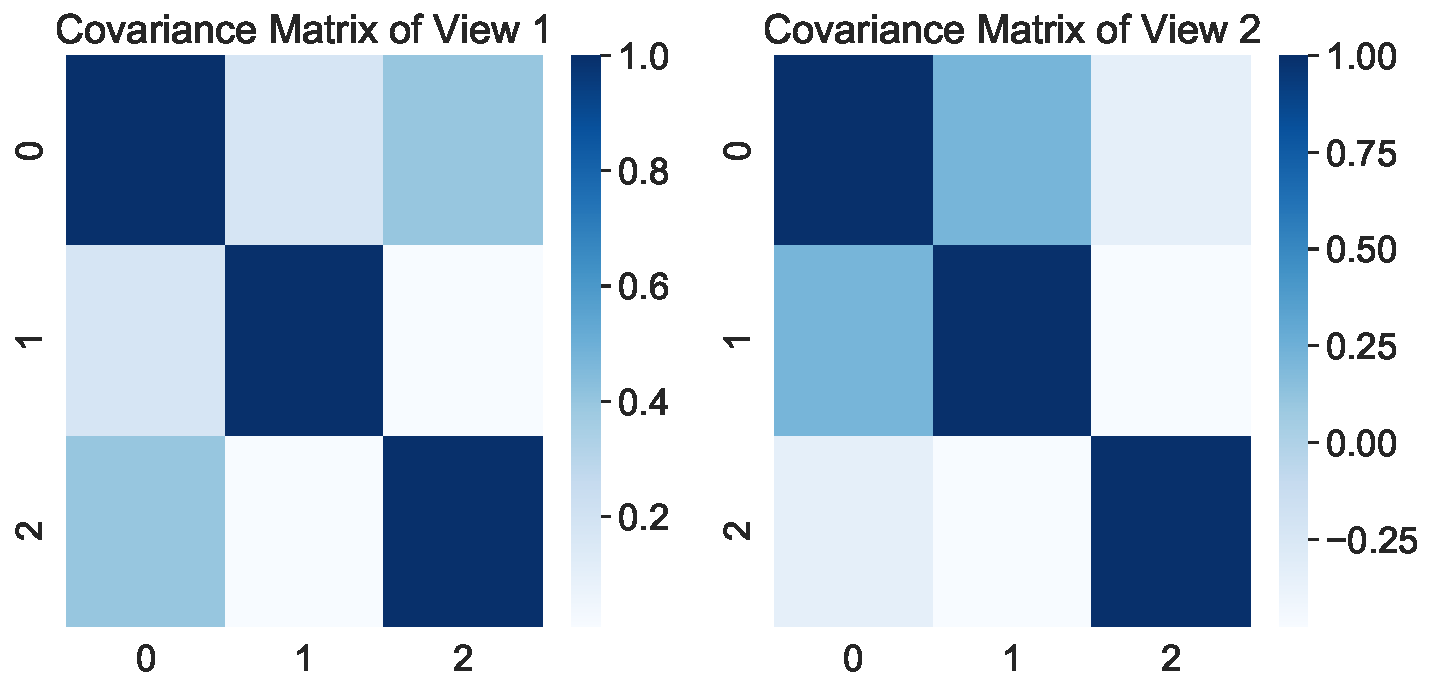
\includegraphics[width=0.8\linewidth]{figures/simulated/explicit/True_Covariance_Correlated.pdf}
    \caption{Example instances of correlated covariance matrices.}\label{fig:covariance-matrices}
\end{figure}

Recalling table \ref{tab:covariance-structures}, note that in the implicit latent variable models, these covariance matrices are precisely the population within-view covariance matrices.
In the explicit latent variable models, these covariance matrices are just the covariance matrices of the noise to which we add the signal covariance matrices.
Nonetheless, for strong enough noise, this process ensures that there are large correlations between features.

\section{Experiment Results}

\subsection{Exploring the Relationship Between Weights and Loadings in CCA Using Simulated Data}

We first present the results of the experiments demonstrating the relationship between weights and \gls{loadings} in simulated data from explicit and implicit latent variable models with identity and non-identity covariance matrices.

For both cases, we plot the true weights and loadings along with the estimated weights and loadings for each model.
We estimate model loadings by multiplying the model weights by the sample within-view covariance matrix following equation \ref{eq:weights-to-loadings}.
This means that the estimated model loadings may not be sparse even when the estimated model weights are sparse and the \textit{population} covariance matrix is identity.

We can also quantify the similarity between the true and estimated weights and \gls{loadings} using the cosine similarity; a measure of the similarity between two vectors that is invariant to the scale of the vectors.
The cosine similarity between two vectors is defined as the cosine of the angle between them \citep{luo2018cosine}.
Since we are indifferent to the direction of the vectors, we take the absolute value of the cosine similarity.
The absolute cosine similarity between two vectors is 1 if they are identical (up top a sign) and 0 if they are orthogonal.

\subsubsection{Implicit Latent Variables (Sparse Weights)}

Figure \ref{fig:implicit-weights-loadings} shows the true and estimated weights and \gls{loadings} for data generated from the implicit latent variable models with sparse weights.
The Elastic net model exhibits no false negatives (i.e. where the true weight is non-zero but the estimated weight is zero) in both cases.
This shows that the Elastic Net CCA model is able to recover the true weights and that the Lasso penalty is indeed inducing sparsity in the weights.
The CCA model appears recover spectrum of the true weights much better for the identity covariance matrices than for the correlated covariance matrices.
This is likely because the multicollinearity introduced makes the learnt weights substantially less stable with respect to a change in the data.

\begin{figure}
\centering
\begin{subfigure}{0.49\linewidth}
\centering
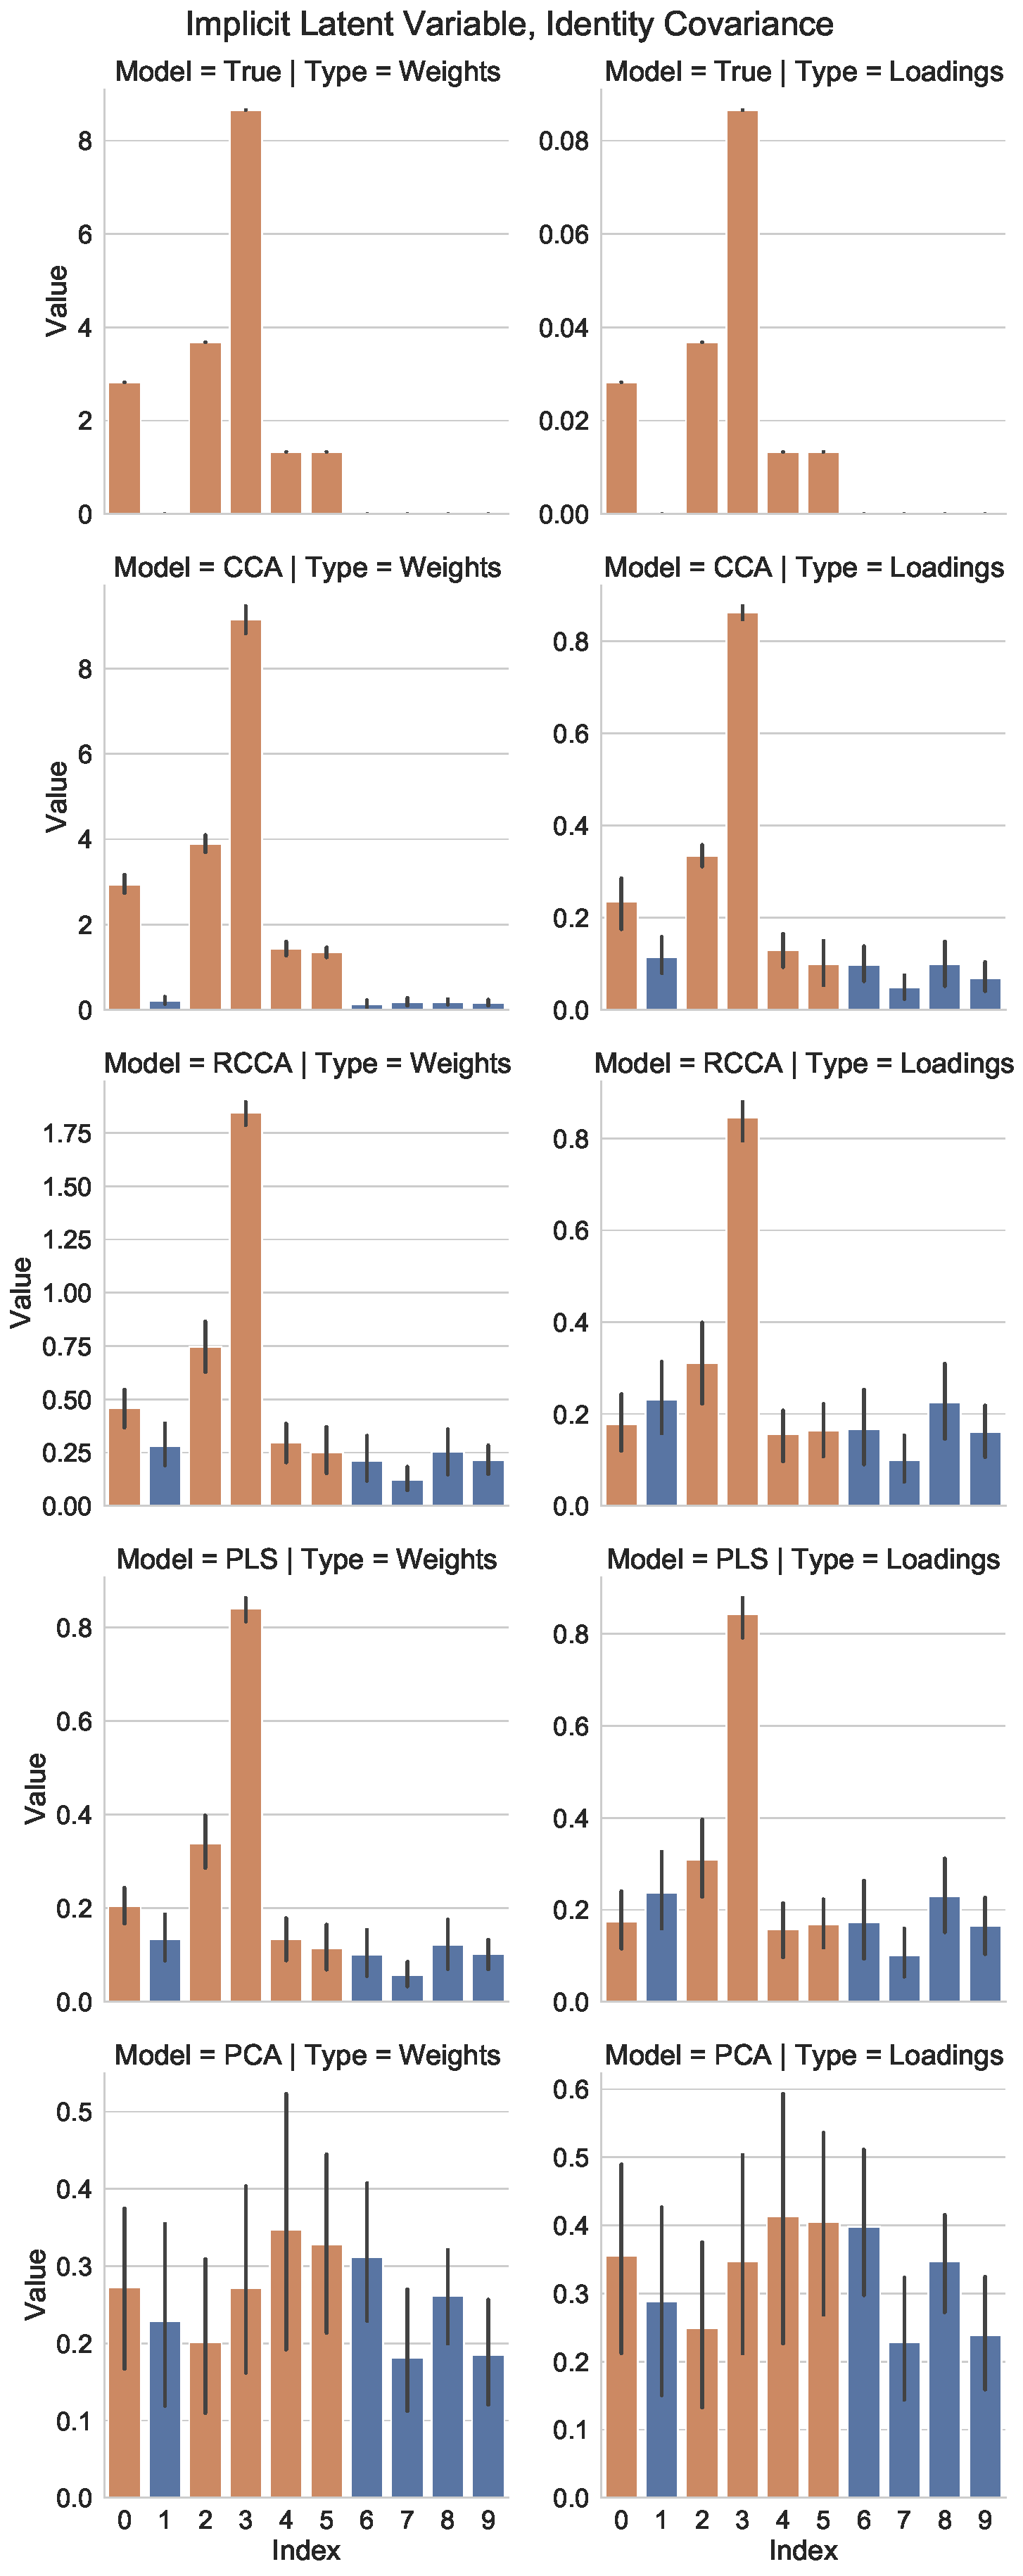
\includegraphics[width=\linewidth]{figures/simulated/implicit/Combined_Weights_Loadings_with_Error_Bars_Identity}
\end{subfigure}
\begin{subfigure}{0.49\linewidth}
\centering
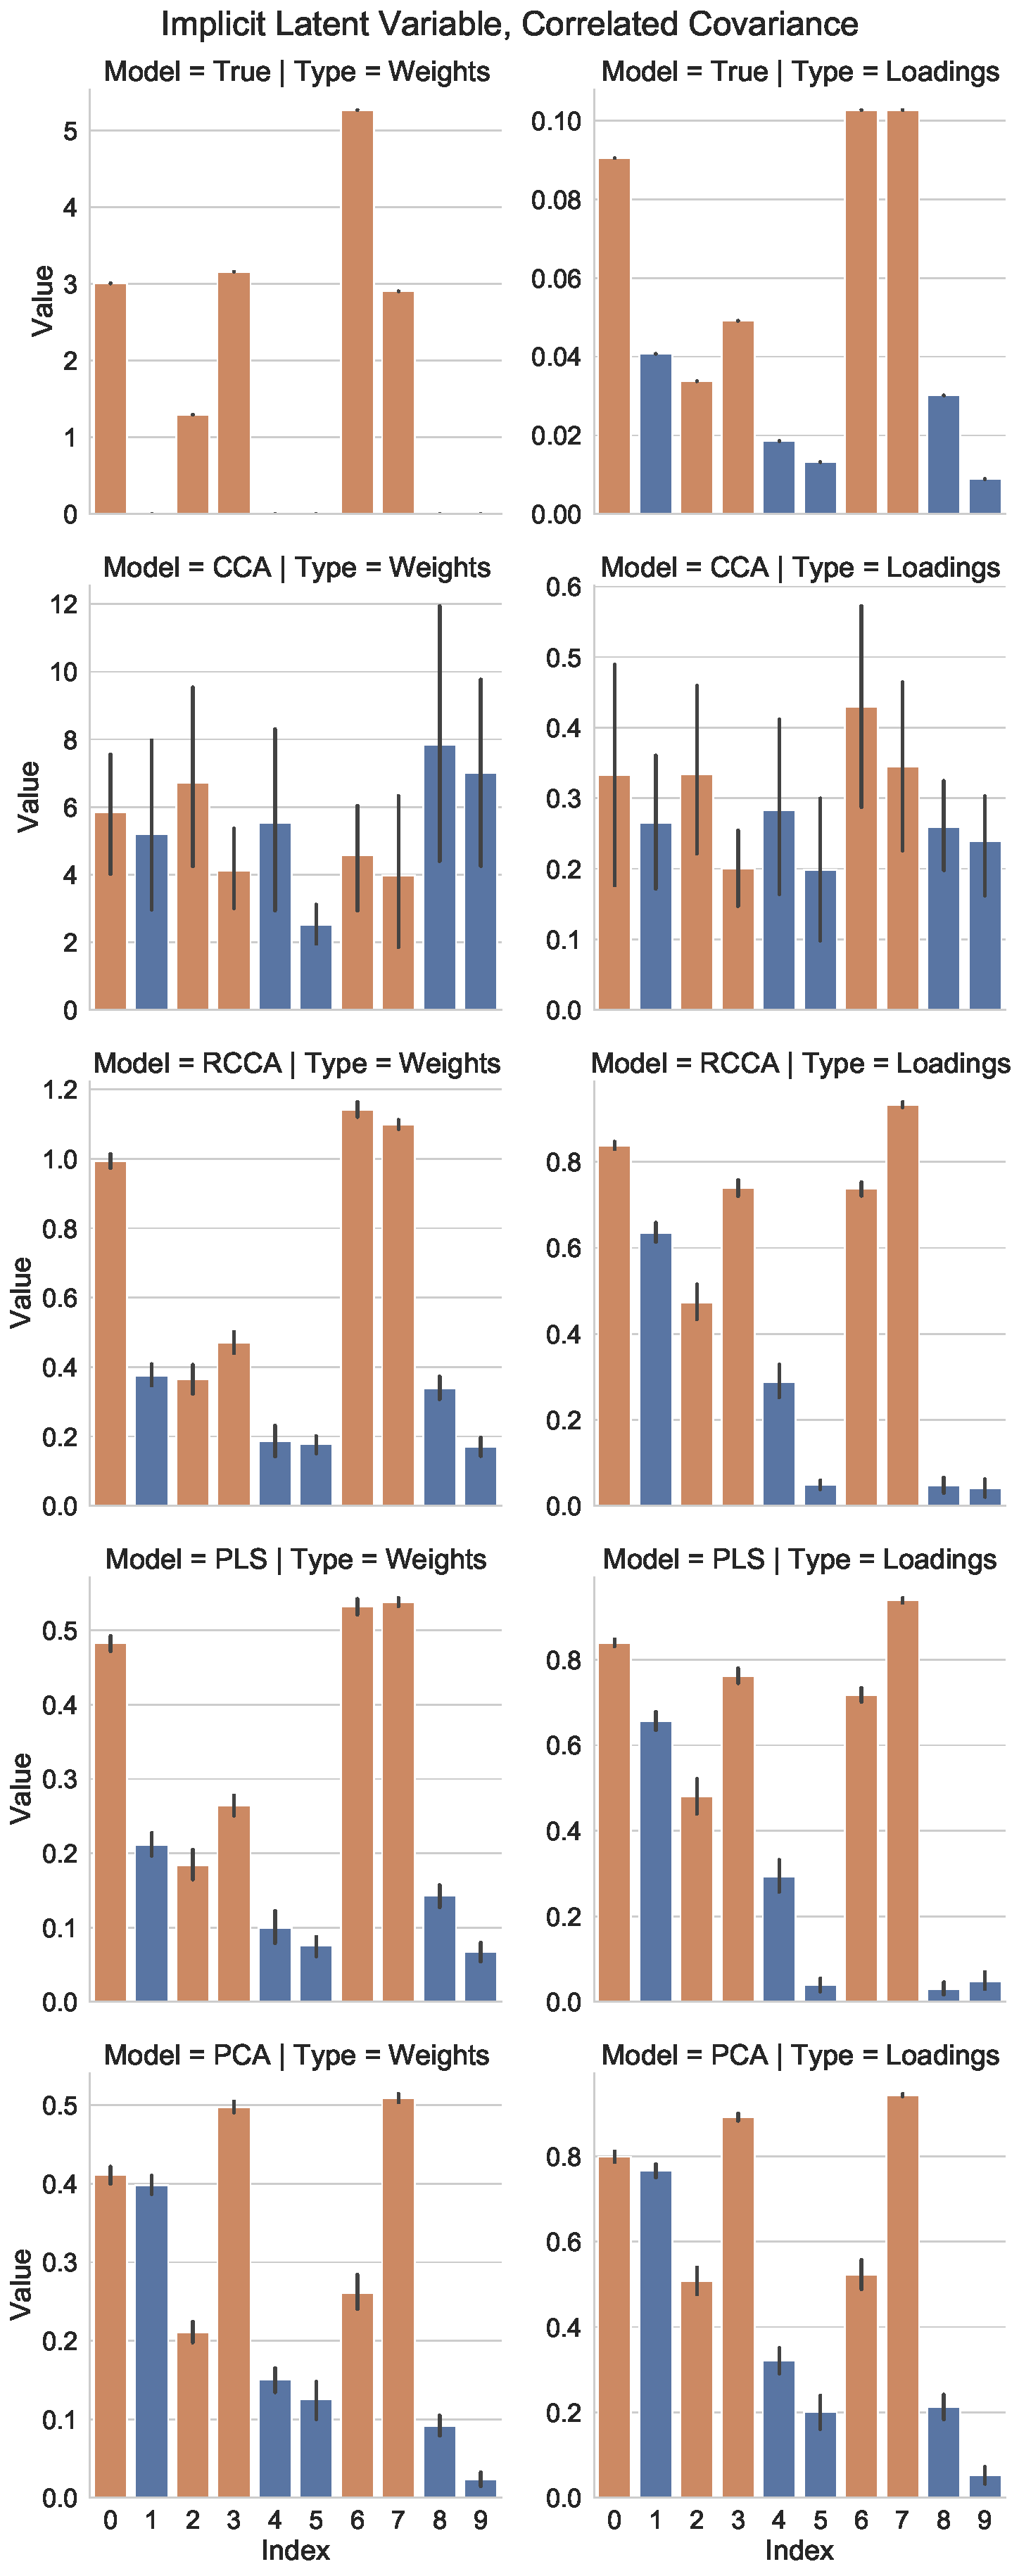
\includegraphics[width=\linewidth]{figures/simulated/implicit/Combined_Weights_Loadings_with_Error_Bars_Correlated}
\end{subfigure}
\caption{Bar plots of the true and estimated weights and \gls{loadings} for data generated from the implicit latent variable models with sparse weights. The left column shows the results for the identity covariance matrices, while the right column shows the results for the correlated covariance matrices.}\label{fig:implicit-weights-loadings}
\end{figure}

We plot the cosine similarity between the true and estimated weights and \gls{loadings} for data generated from the implicit latent variable models with sparse weights in figure \ref{fig:implicit-weights-loadings-cosine}.

\begin{figure}
\centering
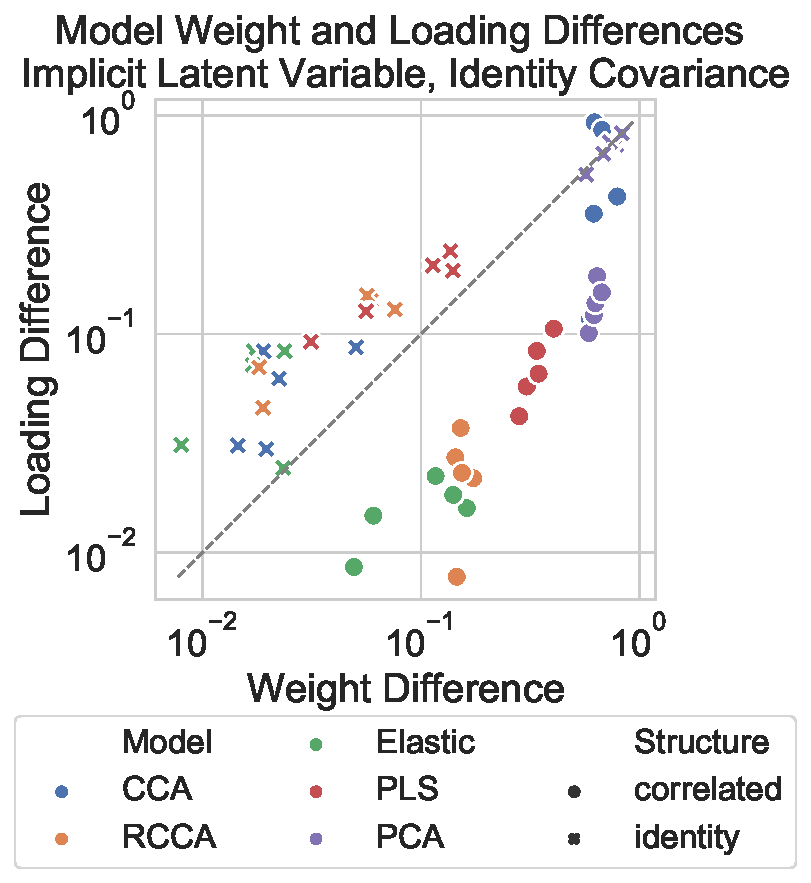
\includegraphics[width=0.8\linewidth]{figures/simulated/implicit/weight_loading_difference}
\caption{Cosine similarity between the true and estimated weights and \gls{loadings} for data generated from the implicit latent variable models with sparse weights. We plot each run as a point on a scatter plot with a log scale. The grey line indicates where the similarity between weights and loadings are equal.}\label{fig:implicit-weights-loadings-cosine}
\end{figure}

Interestingly, we see that for the identity covariance matrices, weight differences are smaller than loading differences.
On the other hand for the correlated covariance matrices, the loading differences are smaller than the weight differences.
This is evidence of the fact that the weights are not identifiable in the implicit latent variable model as suggested by our theory.
Only when the covariance matrices are identity, and when there is only one latent variable, are the weights identifiable.

\subsubsection{Explicit Latent Variables}

Figure \ref{fig:explicit-weights-loadings} shows the true and estimated weights and \gls{loadings} for data generated from the explicit latent variable models with sparse \gls{loadings}.
The left column shows the results for the identity covariance matrices, while the right column shows the results for the correlated covariance matrices.
Once again, the Elastic Net CCA model exhibits no false negatives (i.e. where the true weight is non-zero but the estimated weight is zero) when the noise covariance matrix is identity such that both the weights and \gls{loadings} are sparse.

\begin{figure}
\centering
\begin{subfigure}{0.49\linewidth}
\centering
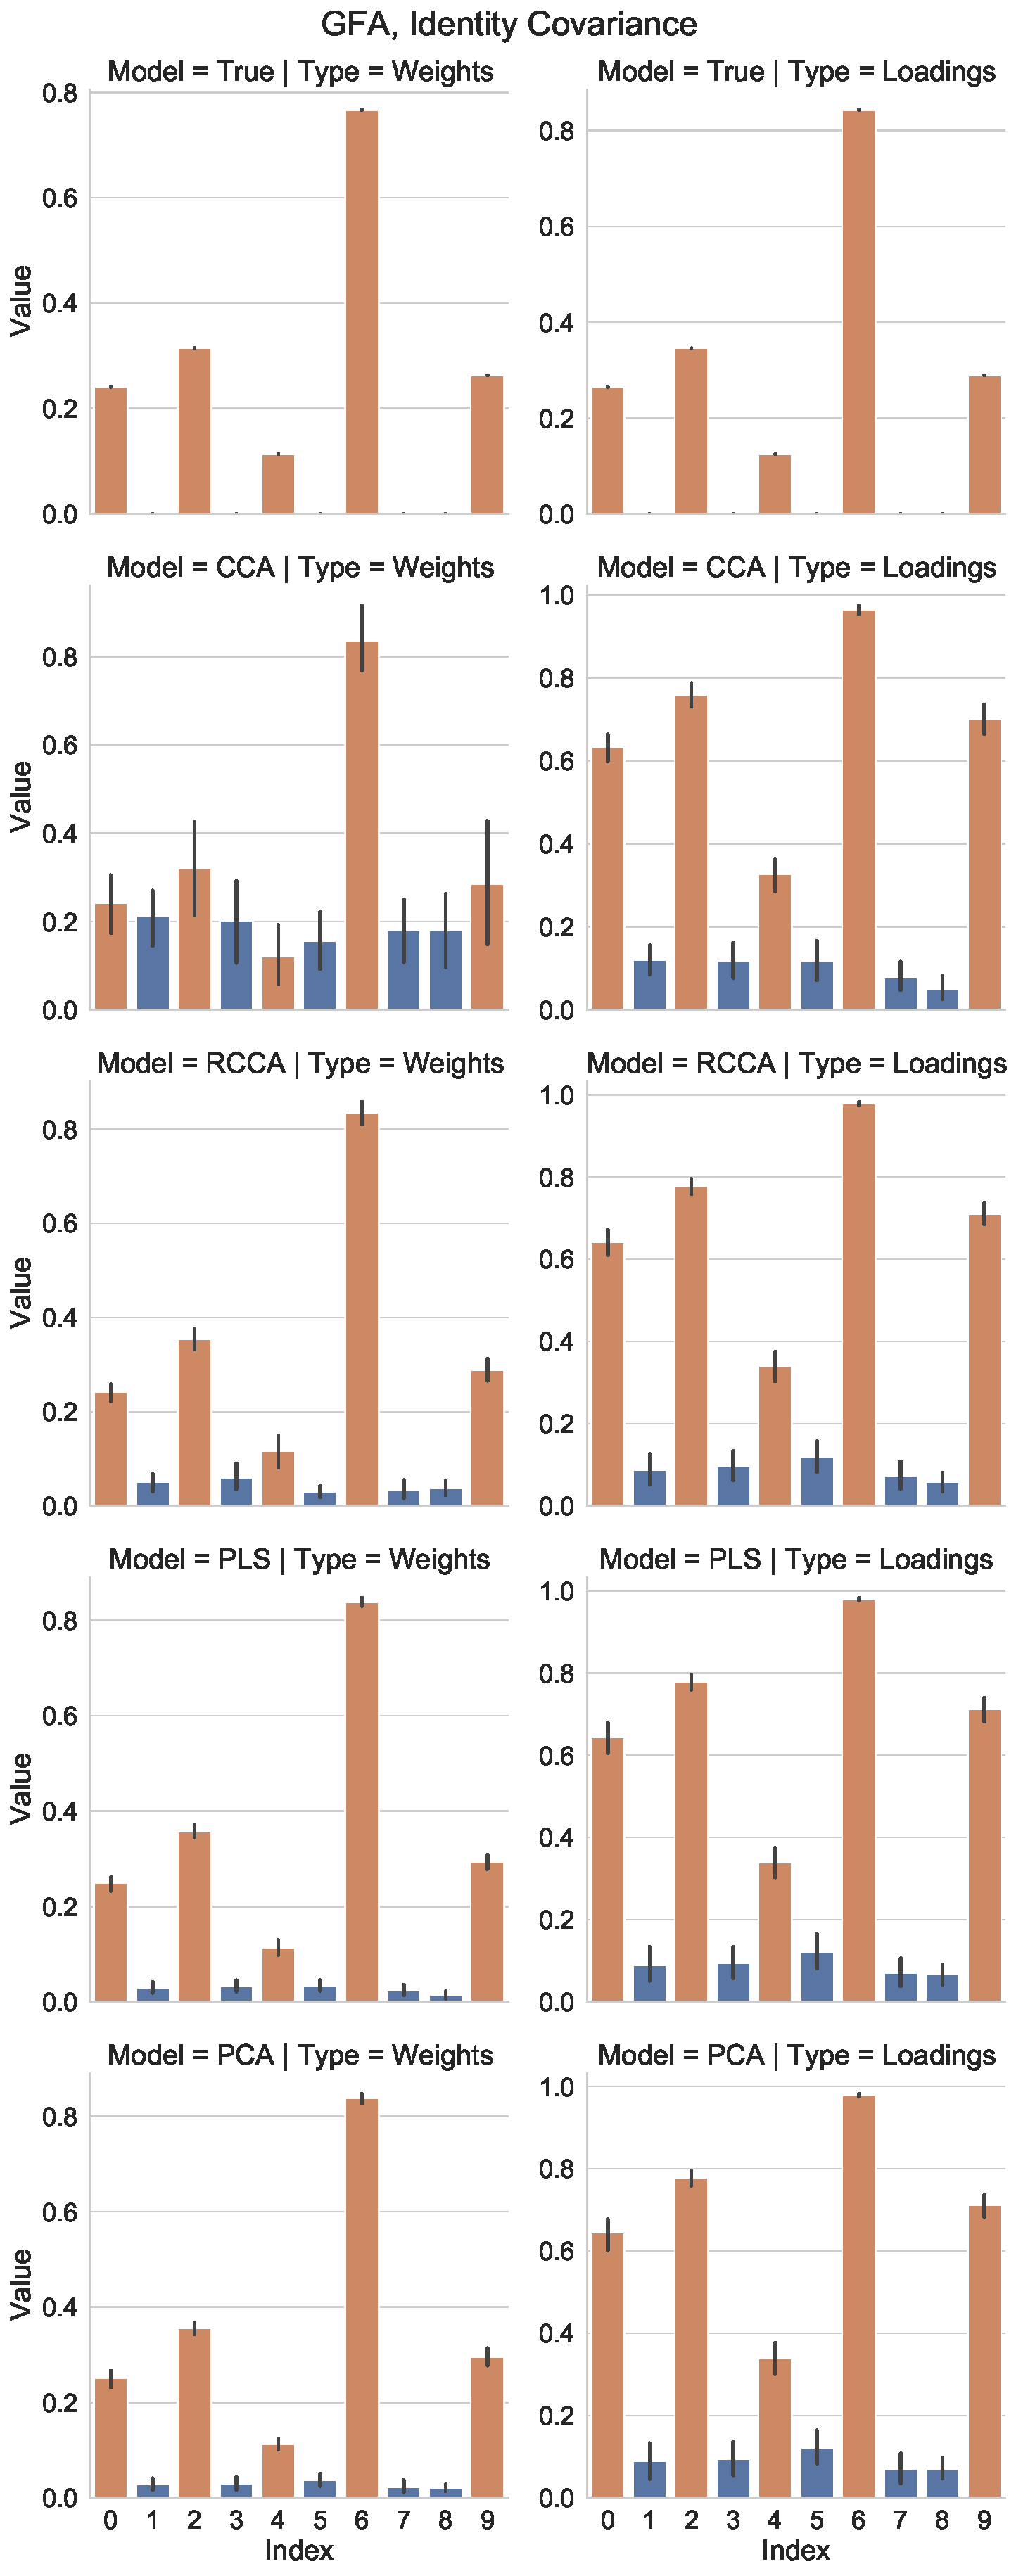
\includegraphics[width=\linewidth]{figures/simulated/explicit/Combined_Weights_Loadings_with_Error_Bars_Identity}
\end{subfigure}
\begin{subfigure}{0.49\linewidth}
\centering
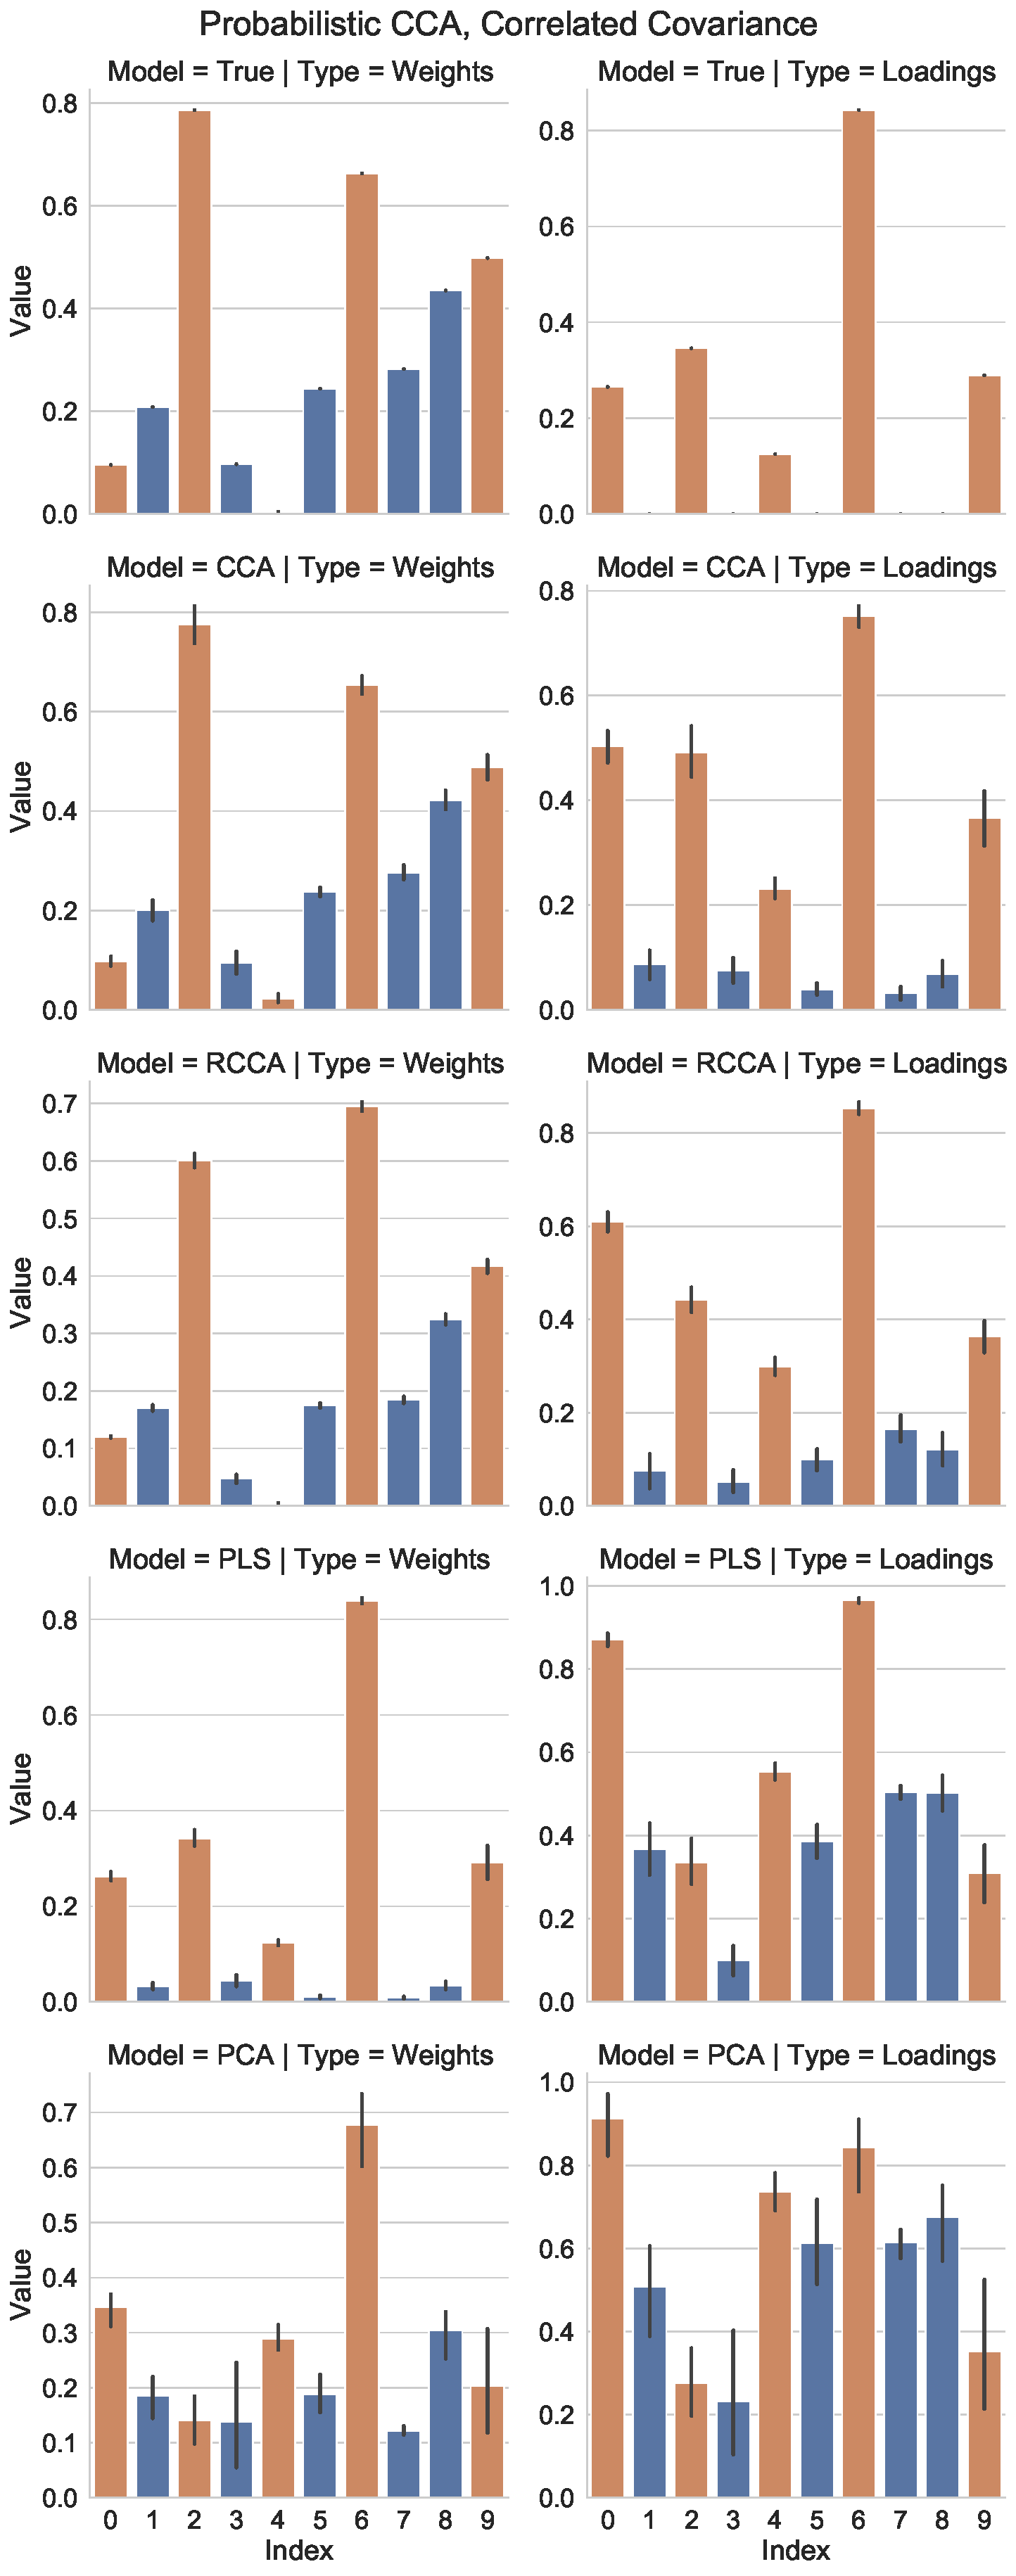
\includegraphics[width=\linewidth]{figures/simulated/explicit/Combined_Weights_Loadings_with_Error_Bars_Correlated}
\end{subfigure}
\caption{Bar plots of the true and estimated weights and \gls{loadings} for data generated from the explicit latent variable models with sparse loadings. The left column shows the results for the identity covariance matrices, while the right column shows the results for the correlated covariance matrices.}\label{fig:explicit-weights-loadings}
\end{figure}

Once again, we can quantify the similarity between the true and estimated weights and \gls{loadings} using the cosine similarity (Figure \ref{fig:explicit-weights-loadings-cosine}).

\begin{figure}
\centering
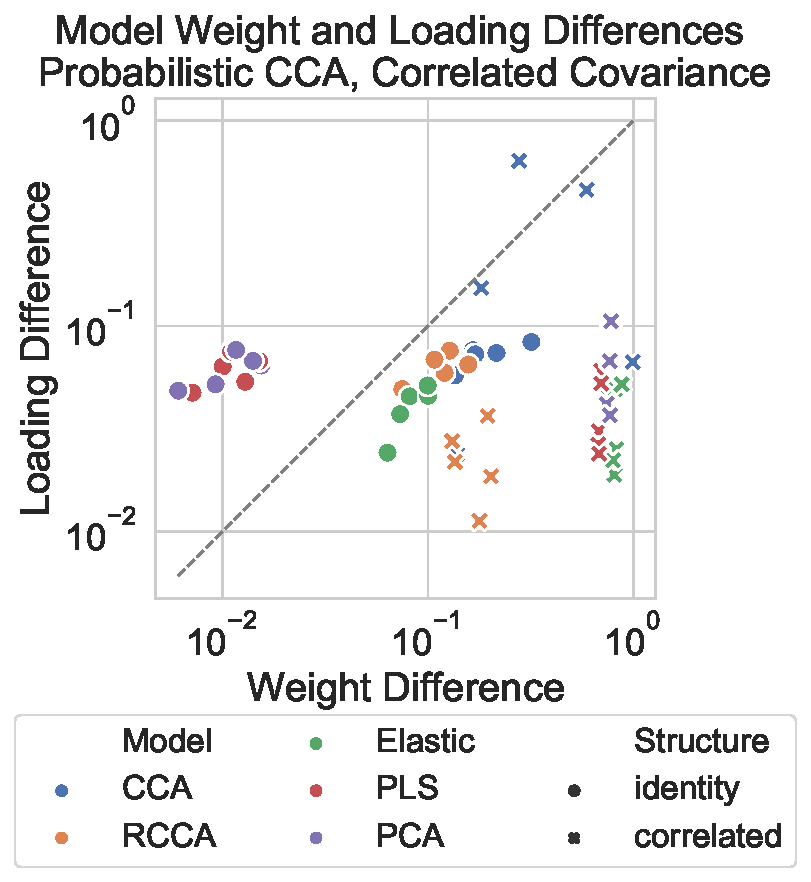
\includegraphics[width=0.8\linewidth]{figures/simulated/explicit/weight_loading_difference}
\caption{Cosine similarity between the true and estimated weights and \gls{loadings} for data generated from the explicit latent variable models with sparse \gls{loadings}. We plot each run as a point on a scatter plot with a log scale. The grey line indicates where the similarity between weights and loadings are equal.}\label{fig:explicit-weights-loadings-cosine}
\end{figure}

Notably, when the noise covariance matrix is correlated, the difference in recovery of the weights is much larger than the difference in recovery of the \gls{loadings}.
Suprisingly, when the noise covariance matrix is identity, the PLS and PCA models appear to better recover the weights than the loadings in this case.

\subsection{Assessing Information Recovery in CCA and PLS Models Under Varying Signal-to-Noise Ratios}

In Figures \ref{fig:snr-scores-identity} and \ref{fig:snr-scores-random} we plot the test correlation (score) varying the signal-to-noise ratio and the number of features under the identity and correlated noise covariance matrices respectively.

In figure \ref{fig:snr-scores-identity}, we can see that the PLS model outperforms all of the Ridge CCA models for all values of the signal-to-noise ratio and dimensionality, though only by a small margin.
The unregeularized CCA model is much worse than even the Ridge CCA model with the smallest regularization.
In this experiment the performance of PLS is directly related to the signal-to-noise ratio.

\begin{figure}
    \centering
    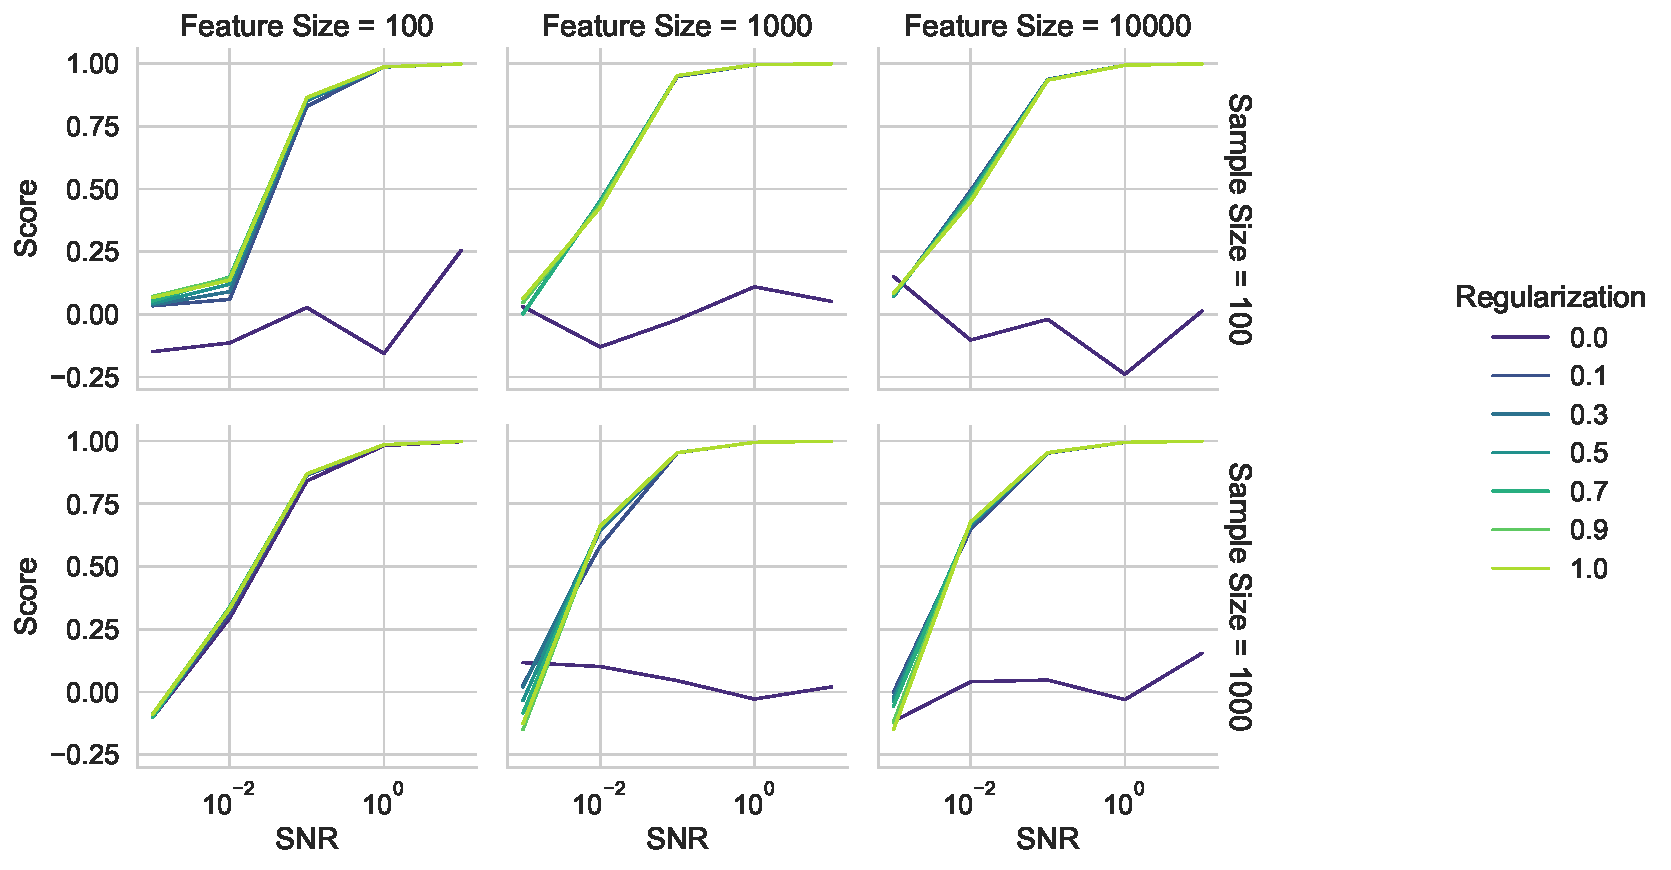
\includegraphics[width=\linewidth]{figures/brain_behaviour_sim/snr_vs_scores_facet_identity}
    \caption{Varying signal to noise ratio with identity covariance matrices. We plot the performance of different levels of Regularized CCA from 0 (CCA) to 1 (PLS) for different sample sizes. }\label{fig:snr-scores-identity}
\end{figure}

In figure \ref{fig:snr-scores-random}, we see a totally different picture.
The PLS model is now outperformed by the Ridge CCA model with the smallest regularization.
While CCA is still the worst performing model, PLS is now much worse across signal-to-noise ratios and dimensions than any of the Ridge CCA models.
This suggests that the PLS model is not able to recover anything like the true signal when the covariance matrices are correlated.


In this experiment it is also clear that the signal-to-noise ratio must be higher to obtain the same performance with higher dimensional data.
It is interesting that performance of the Ridge CCA improves across the board with lower regularization.


\begin{figure}
    \centering
    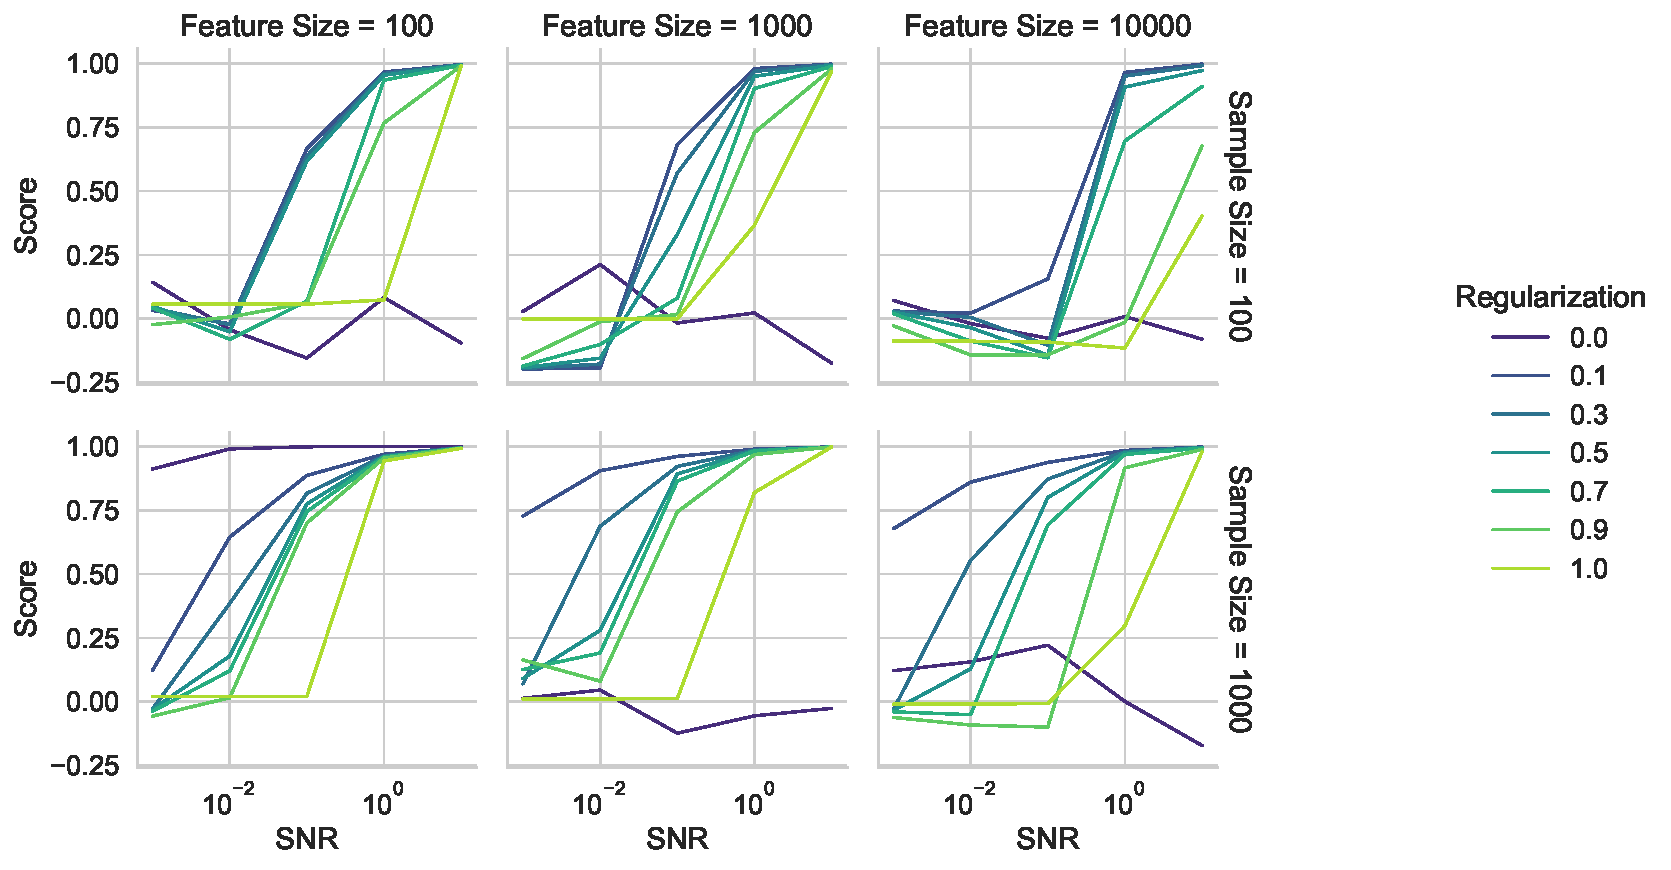
\includegraphics[width=\linewidth]{figures/brain_behaviour_sim/snr_vs_scores_facet_random}
    \caption{Varying signal to noise ratio with correlated covariance matrices. We plot the performance of different levels of Regularized CCA from 0 (CCA) to 1 (PLS) for different sample sizes.}\label{fig:snr-scores-random}
\end{figure}

\section{Discussion and Limitations}

\subsection{Revisiting the results from chapter \ref{ch:als}}

In appendix \ref{appendix:loadings}, we revisit the results from chapter \ref{ch:als} in the context of the theoretical results from this chapter. While they are not the focus of this chapter, they provide a useful comparison and point of reference for the results in this chapter.

\subsection{Future Work}

Given our theoretical observations in this chapter, a natural question to ask is whether we can construct a regularization functional that imposes sparsity on the \gls{loadings} (instead of the weights).
The answer is yes, but it is not straightforward and in the small sample setting, it is not clear that it is a good idea.
The principle would be much the same as the Lasso, but we would need to use the sample covariance matrix to define the norm:

\begin{align}
    P(W)=\|W\|_1 \\
    P(L)=\|\hat{\Sigma}U\|_1
\end{align}

Which imposes an L1 penalty on the \gls{loadings} via an L1 penalty on the \gls{weights} multiplied by the sample covariance matrix.
We could in principle apply the soft-thresholding operator to the estimated loadings.
However we would need to be careful to ensure that the sample covariance matrix is invertible in order to get back to the weights.
This is of course not guaranteed in the small sample setting.

\subsection{Conclusion}

In this chapter, we explored the relationship between weights and loadings in CCA models from both theoretical and empirical perspectives. We unified methods for generating simulated multiview data using implicit and explicit latent variable models, providing a framework for understanding the properties of CCA and PLS models.

Through a rigorous mathematical argument, we demonstrated that loadings are invariant to columnwise transformations of the data matrix, while weights are not. This invariance property makes loadings a more reliable choice for interpreting CCA models, as the weights can be arbitrarily set by scaling the data matrix or adding linear combinations of columns.

Our experiments using simulated data provided empirical evidence supporting the theoretical findings. We showed that the recovery of true weights and loadings depends on the underlying covariance structure and the choice of regularization. The results highlighted the importance of considering the signal-to-noise ratio and dimensionality when applying CCA and PLS models to real-world datasets.

Overall, this chapter contributes to a better understanding of the behavior and interpretation of CCA models, providing valuable insights for researchers and practitioners working with multiview data. The findings emphasize the importance of considering the invariance properties of loadings and the impact of covariance structure and regularization on model performance. Future research could explore the extension of these insights to more complex data scenarios and the development of efficient algorithms for imposing sparsity on loadings in CCA models.